\documentclass[../main/report.tex]{subfiles}
\begin{document}

\section{Power}

The system is powered by a 5V mini USB.
This connection powers two voltage regulator circuits.
Respectively, the 1.2V wire that powers the FPGA (excluding the I/O banks) and the 3.3V power plane that powers up the rest of the machine.
The 5 volt USB connection has a backup solution in the form of a header through which it passes immediately after entering the PCB.
This is done so that the incoming electricity can easily be probed for voltage level and also so that in case the USB connection fails, an external power supply can be connected to the board.

\begin{figure}[H]
	\centering
	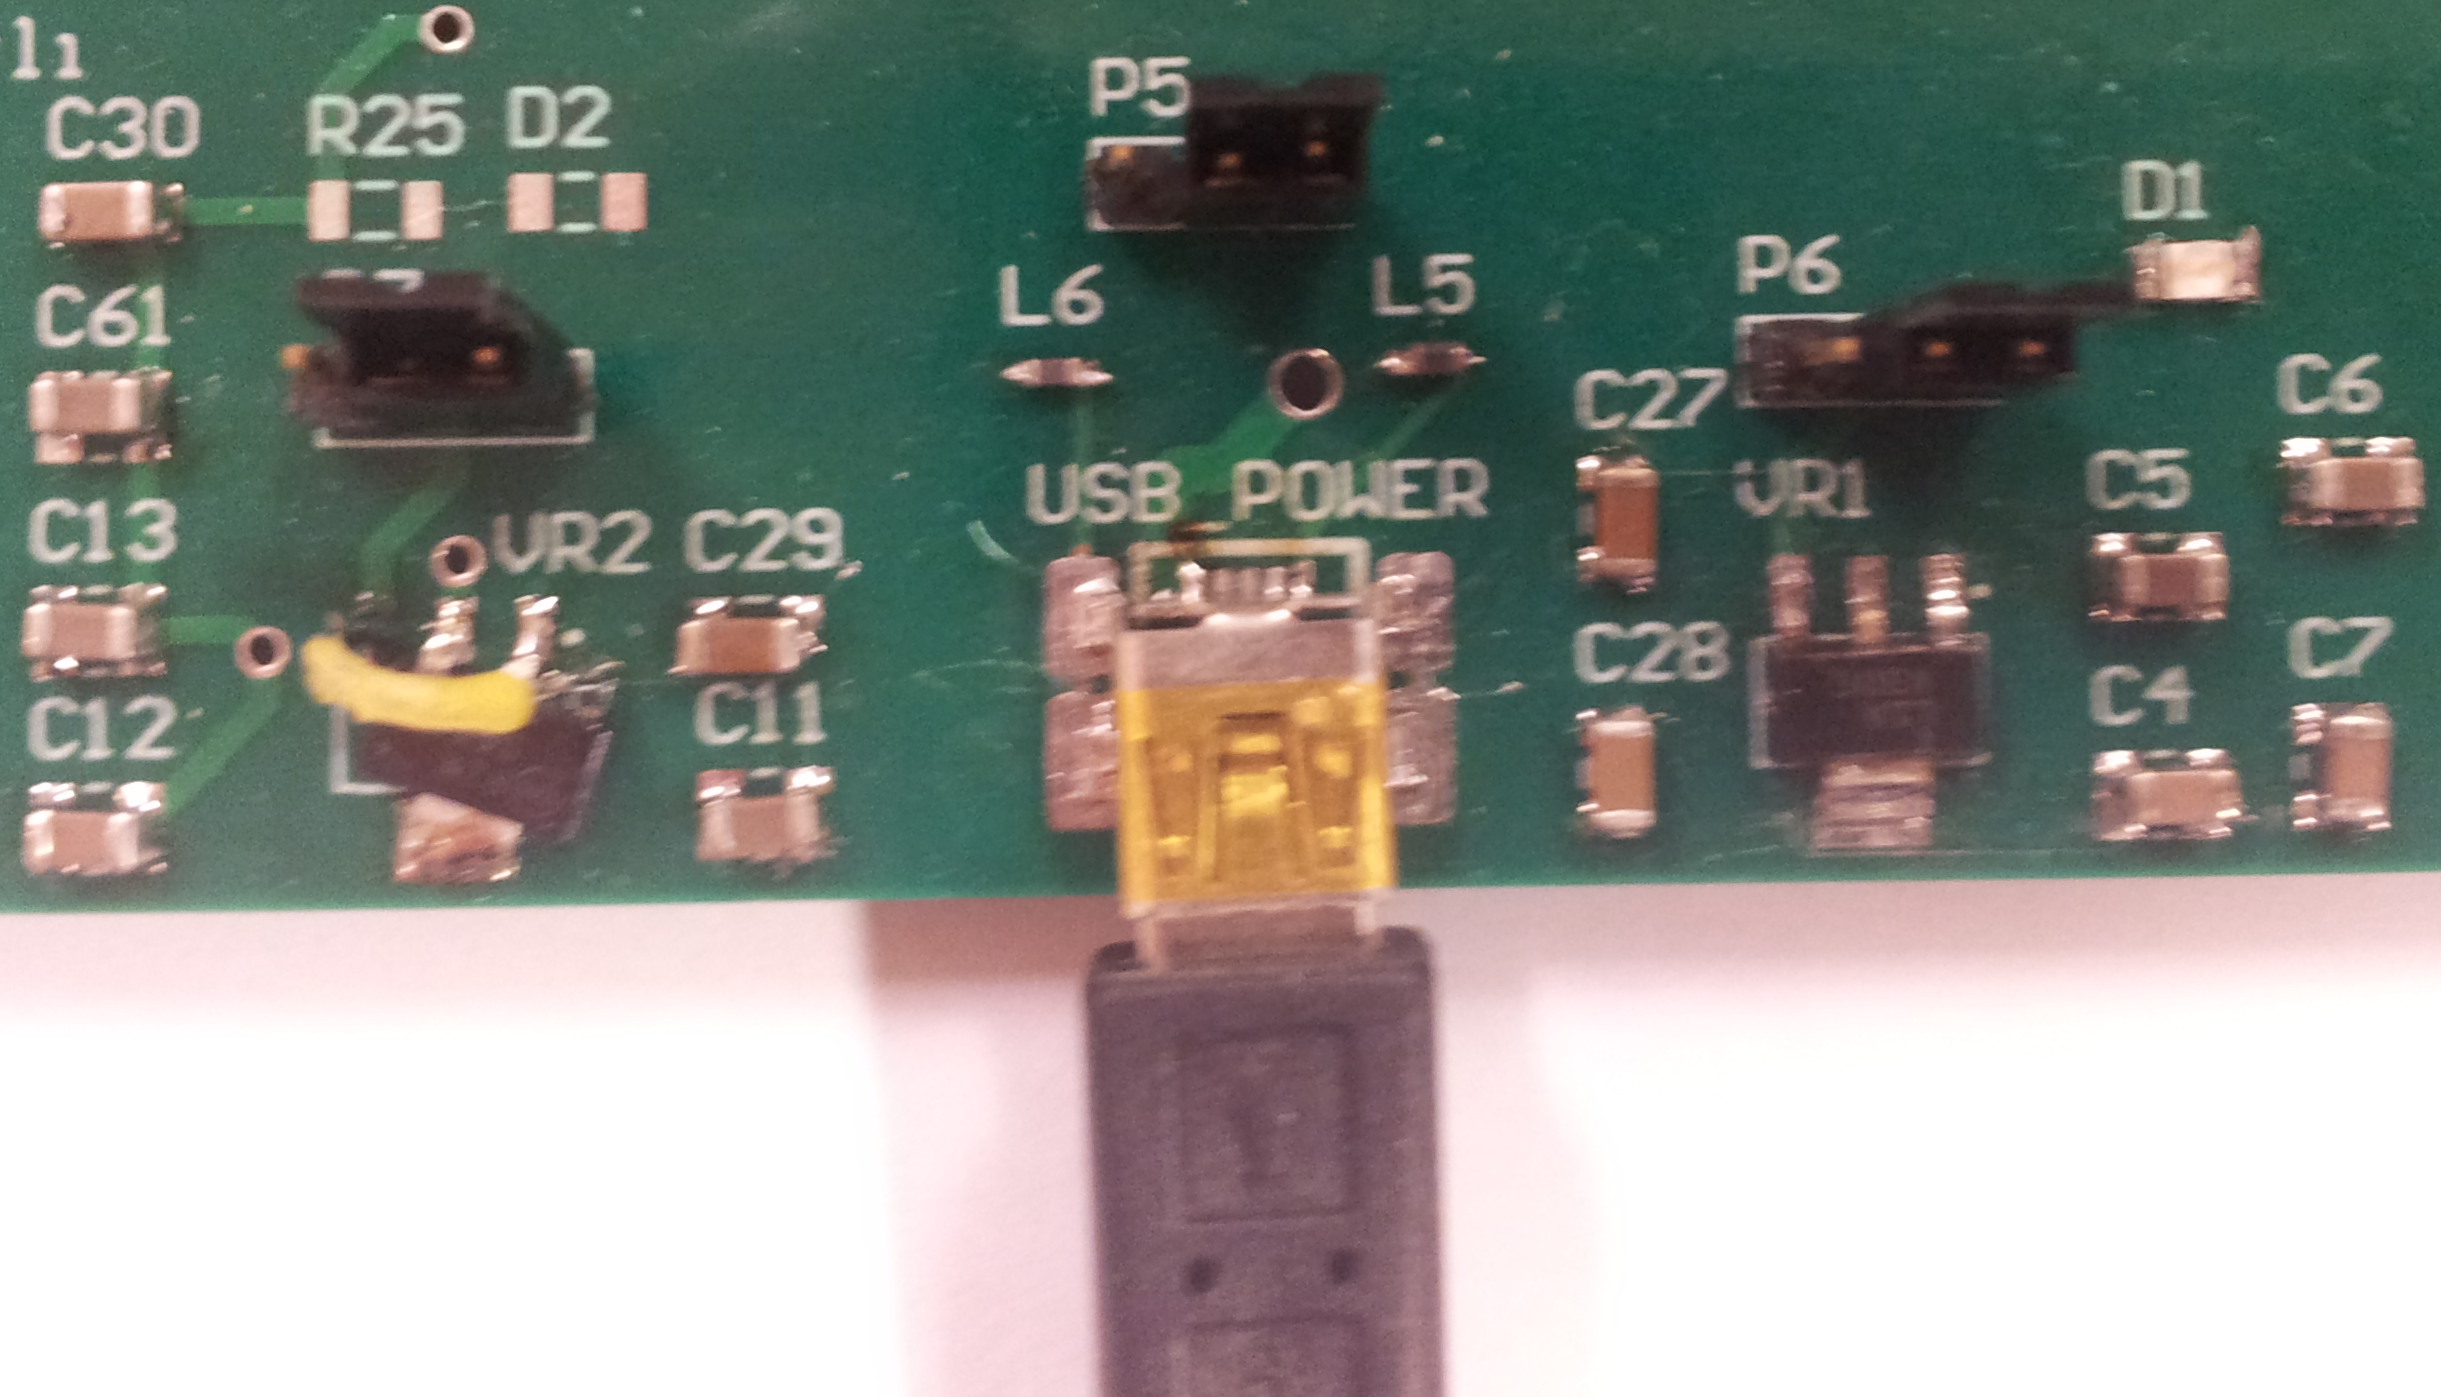
\includegraphics[width=0.65\textwidth]{../pcb/assets/power.png}
	\caption{Picture of the physical power circuit, where P5 is the header on which an external power source can be connected}
	\label{fig:power-circuit}
\end{figure}

\end{document}
